\clearpage
\section{problem 5}
Both datasets use an 80/20 split with seed 42. Each PyTorch model is trained directly on its full training set for 200 epochs with fixed hyperparameters, without cross-validation. Features are standardized using training data only. Classification probabilities are clipped to $[10^{-6},1-10^{-6}]$ before computing BCE; gradient norms are clipped at 5.

\paragraph{Classification ($n_{\mathrm{train}}=455$, $n_{\mathrm{test}}=114$).}
\begin{center}
  \begin{tabular}{lrrr}
    \hline
    Model & Correct & Test accuracy & $\Delta$ accuracy \\
    \hline
    sklearn logistic (L2) & 112/114 & 0.9825 & +0.0000 \\
    PyTorch logistic (SGD) & 110/114 & 0.9649 & -0.0175 \\
    PyTorch probit (SGD) & 109/114 & 0.9561 & -0.0263 \\
    \hline
  \end{tabular}

\end{center}

\paragraph{Classification (a).} SGD: 200 epochs, batch size 64, initial learning rate 0.05, momentum 0. The sigmoid model has test accuracy 96.49\%, which is 1.75 percentage points lower than the sklearn baseline. The PyTorch model minimizes BCE without a penalty; the sklearn baseline uses L2 regularization.

\paragraph{Classification (b).} SGD: 200 epochs, batch size 64, initial learning rate 0.05, momentum 0. Replacing sigmoid with the standard normal CDF gives test accuracy 95.61\%, which is 2.63 percentage points lower than the sklearn baseline. Both implementations use the same clipped BCE.

\begin{center}
  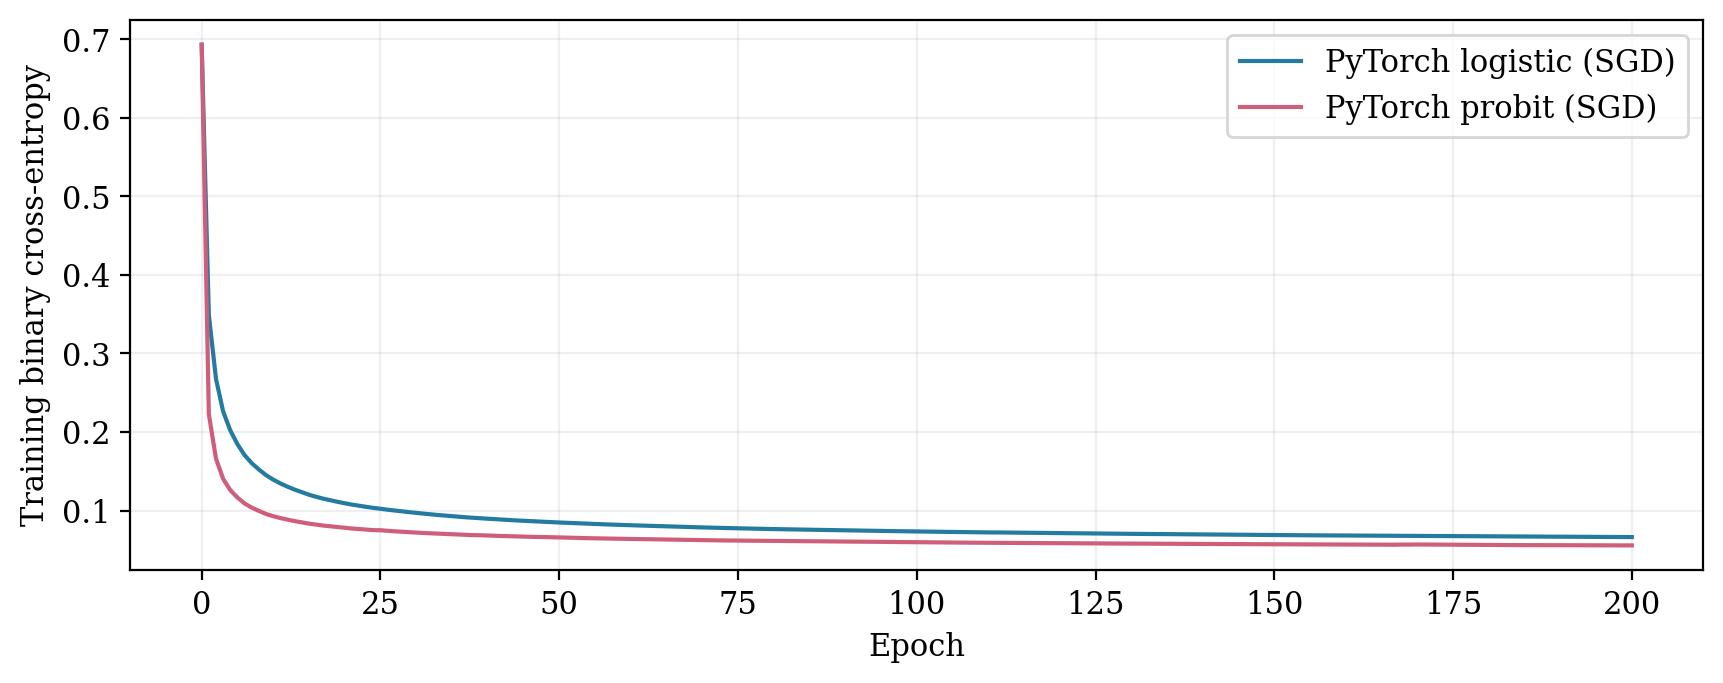
\includegraphics[width=0.9\textwidth]{problem5_autodiff/figures/classification_loss.png}
\end{center}

\clearpage
\paragraph{Regression ($n_{\mathrm{train}}=85$, $n_{\mathrm{test}}=22$).}
\begin{center}
  \begin{tabular}{lrr}
    \hline
    Model & Test MAE (m) & $\Delta$ MAE (m) \\
    \hline
    sklearn linear & 0.195393 & +0.000000 \\
    PyTorch linear (MSE, SGD) & 0.195232 & -0.000161 \\
    PyTorch linear ($t_5$ NLL, SGD) & 0.194035 & -0.001358 \\
    \hline
  \end{tabular}

\end{center}

\paragraph{Regression (a).} SGD: 200 epochs, batch size 32, initial learning rate 0.03, momentum 0. The linear model trained with MSE has test MAE 0.195232 m, which is 0.000161 m lower than the sklearn baseline. A finite number of stochastic updates can produce a small difference from the least-squares baseline.

\paragraph{Regression (b).} SGD: 200 epochs, batch size 32, initial learning rate 0.03, momentum 0. Minimizing the Student-$t$ negative log-likelihood with $\nu=5$ and fixed scale 1 gives test MAE 0.194035 m, which is 0.001358 m lower than the sklearn baseline. ALE remains in its original units.

\begin{center}
  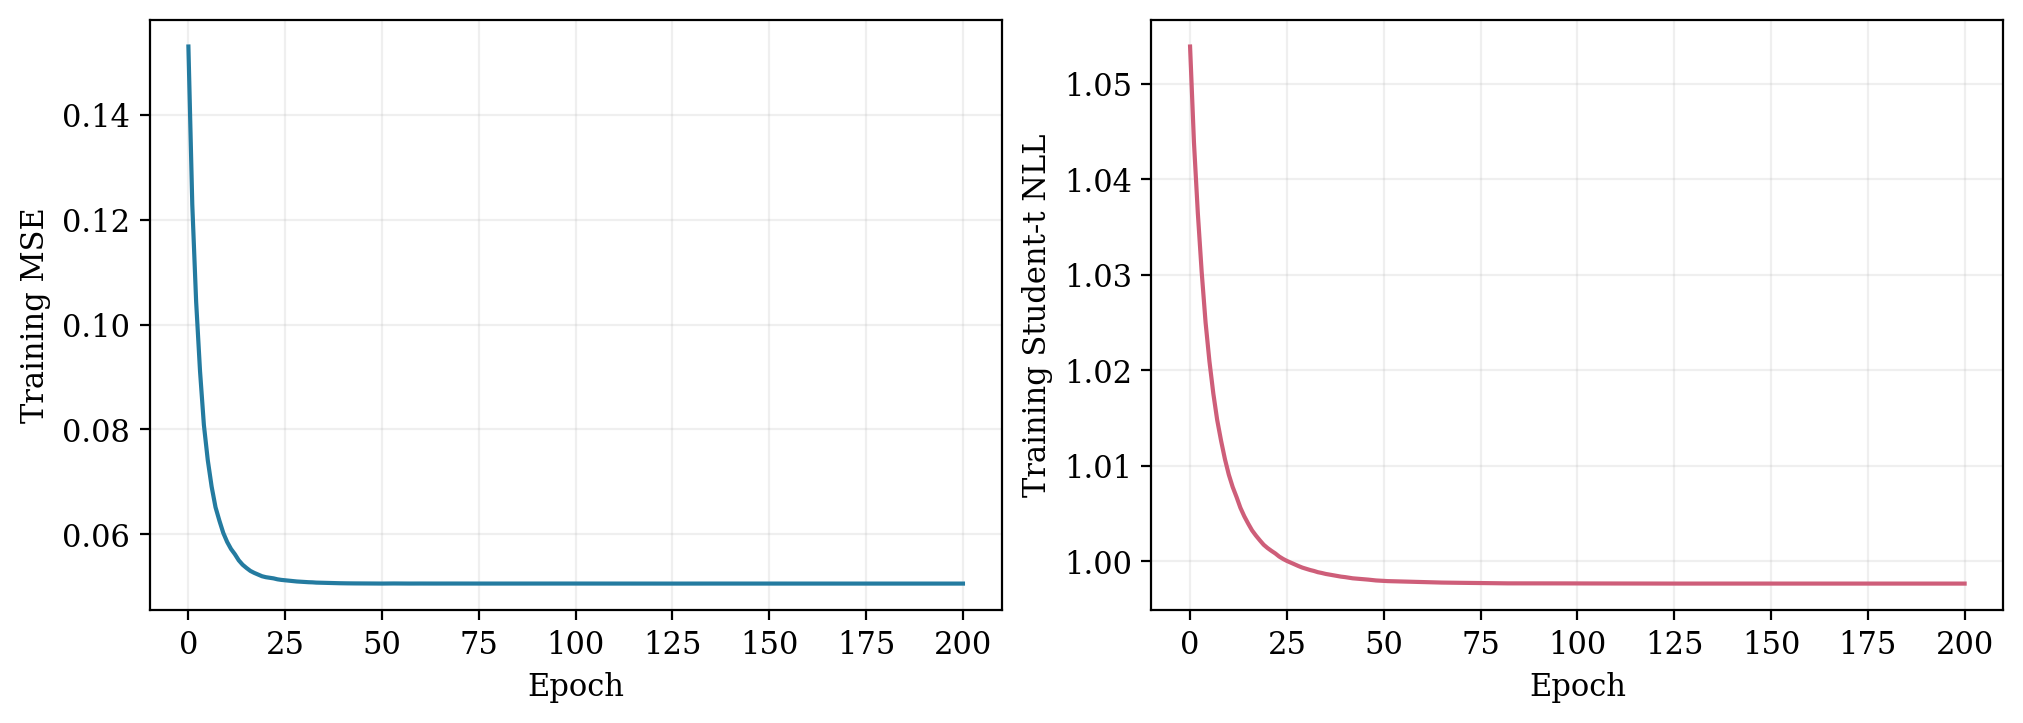
\includegraphics[width=\textwidth]{problem5_autodiff/figures/regression_loss.png}
\end{center}
